\documentclass{article}
\usepackage[utf8]{inputenc}
\usepackage[T1]{fontenc} % das Trennen der Umlaute
\usepackage[ngerman]{babel}
\usepackage{colortbl}
\usepackage{microtype}
\usepackage{graphicx}
\usepackage{grffile}
\usepackage{siunitx}  % für Einheiten
\usepackage{hyperref}
\usepackage{amsmath}
\sisetup{locale = DE,  
	separate-uncertainty,  
	range-units = brackets,  
	list-units = single,  
	per-mode=symbol-or-fraction} 
%\usepackage{subfig}
\usepackage{wrapfig}
\usepackage{tikz}
\usetikzlibrary{shapes}
\usepackage{xspace}

%-----------------------------------------------------------------------
%	BIBLIOGRAPHY
%-----------------------------------------------------------------------
\usepackage[style=numeric]{biblatex}
\addbibresource{Bibliographiedatei.bib}
%-----------------------------------------------------------------------


\graphicspath{{Figures/}}

\setlength{\parindent}{0em} 

\title{Dokumentation des BitConnector v3X}
\author{Michael Krause \\CC BY-SA 4.0 (except logo)}

\date{\today}


\begin{document}
\maketitle
%\begin{figure}[!h]
%	\centering
%	
\includegraphics[scale=0.06]{Logo}
%\end{figure}

%\thispagestyle{empty}
%\setlength{\unitlength}{1mm}
\begin{picture}(0,0)
\put(270,38){
\includegraphics[scale=0.10]{Logo}}
\end{picture} %

\section{Einführung}
Die noch immer andauernden Bemühungen der mikrokosmischen Minimierung von integriertern Schaltkreisen hat Integrationsdichten hervorgebracht, die traditionelle Schaltkreise wie einzelne Register, Zähler, ALUs oder Multiplexer vom Markt verschwinden ließen. Aus der Sicht des Endkonsumentenmarktes mag dieser Schritt folgerichtig sein, jedoch gibt es jenseits dessen noch immer das Bedürfnis auf der Register-Transfer Ebene oder darunter, Logikschaltkreise zu modellieren und zu realisieren. Dieses Bedürfnis kann beispielsweise der akademischen Lehre, dem Wunsch nach Parallelisierung oder der Vorgabe zeitkritischer Anwendungen entspringen. Obwohl es diesbezüglich eine Vielzahl von FPGAs und CPLD-Typen zur Abhilfe gibt, gestaltet sich der prototypische Aufbau auf einem Steckbrett mit Hilfe dieser Chips als als nahezu unmöglich. Derartige Chips besitzen meist eine Vielzahl an Pins, die nicht im Dual in-line package (DIP) vorliegen. Der BitConnector versucht dieses Problem zu lösen.

\vspace{0.5cm}

%%Freiheitsgrade ....

\begin{wrapfigure}[14]{l}{0.50\textwidth}
		\vspace { -15pt }
	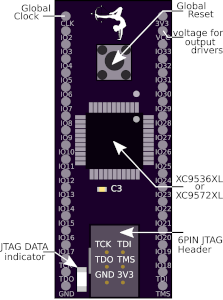
\includegraphics[scale=0.3]{BitConnector6P} 
	\caption{BitConnector v3X}
	\label{fig:}
\end{wrapfigure}

Der BitConnector ist ein \textbf{C}omplex \textbf{P}rogrammable \textbf{L}ogic \textbf{D}evice, kurz \textbf{CPLD} Board, das für den  hardwarebasierten, digitalen Prototypenentwurf auf einem Steckboard optimiert wurde und zudem gesockelt auf andere Platinen aufgesetzt werden kann. Das Board ist so entworfen, dass es einen klassischen DIP Chip mit 2,54 mm Rastermaß und 2 * 20 Pins nachbildet. Konfigurationen, die etwa in einer HDL vorliegen, werden mittels JTAG übertragen und dauerhaft auf dem CPLD gespeichert.
 

\section{Eckdaten} 

BitConnector Board-Spezifikation
\begin{itemize}
	\item \textit{Anzahl der frei beschaltbaren Ein/Ausgänge:} \hspace{0.3cm} 33
	\item \textit{Gesamtanzahl der Pins:} \hspace{3.6cm} 2 Reihen * 20 Pins (2,54mm)
	\item \textit{kompatible CPLD-Varianten}: \hspace{2.8cm} XC95\textbf{72}XL sowie XC95\textbf{36}XL
	\item Max. Produktterme: \hspace{4.1cm} 1600 bei 72XL/800 bei~36XL
	\item \textit{IC-Package}: \hspace{5.3cm} VQ44 
\end{itemize}

Absolute, maximale Belastbarkeit:
\begin{itemize}
	\item \textit{Versorgungsspannung bezogen auf GND:} \hspace{1cm} -0,5V bis 4V
	\item \textit{Eingangsspannung bezogen auf GND:} \hspace{1.45cm} -0,5V bis 5,5V
	\item \textit{Max. Stromfluss bei max. 70 \si{\celsius} Chiptemp.}:\hspace{0.6cm} $\approx1,6A$ (siehe Kapitel \ref{sec:max_I})
\end{itemize}

Es wird empfohlen, Spannungen über und unter 3,3V($\pm 0,3V$) zu vermeiden!

\section{Pinbelegung BitConnector v3X}
\label{sec:Pins}

\begin{minipage}{0.55\textwidth}
	%\begin{table}[h]
	\begin{tabular}{l|c|c|l}
		Nr & DIP-links	& CPLD-Pin & Bemerkung\\
		\rowcolor[gray]{.8}	1 & CLK		& 1 &	GCK3\\
		2 & IO2		& 2 &\\
		\rowcolor[gray]{.8}	3 & IO3		& 3 &\\
		4 & IO4		& 5 &\\
		\rowcolor[gray]{.8}	5 & IO5		& 6 &\\
		6 & IO6		& 7 &\\
		\rowcolor[gray]{.8}	7 & IO7		& 8 &\\
		8 & IO8		& 12 &\\
		\rowcolor[gray]{.8}	9 & IO9		& 13 &\\
		10 & IO10	& 14 &\\
		\rowcolor[gray]{.8}	11 & IO11	& 16 &\\
		12 & IO12	& 18 &\\
		\rowcolor[gray]{.8}	13 & IO13	& 19 &\\
		14 & IO14	& 20 &\\
		\rowcolor[gray]{.8}	15 & IO15	& 21 &\\
		16 & IO16	& 22 &\\
		\rowcolor[gray]{.8}	17 & IO17	& 23 &\\
		18 & TCK		& 11 &	JTAG\\
		\rowcolor[gray]{.8}	19 & TDO		& 24 &	JTAG\\	
		20 & GND		& 17,25,4 & 	 
	\end{tabular}
	%\end{table}
\end{minipage}
\begin{minipage}{0.2\textwidth}
	\begin{tabular}{||c|c|l}
		DIP-rechts	& CPLD-Pin & Bemerkung\\
		\rowcolor[gray]{.8}	3V3		& 15,35 &	V\textsubscript{ccINT} \\
		VCC		& 26 & 		V\textsubscript{ccIO}\\
		\rowcolor[gray]{.8}	IO33	& 44 &		GCK2\\
		IO32	& 43 &		GCK1\\
		\rowcolor[gray]{.8}	IO31	& 42 &\\
		IO30	& 41 &\\
		\rowcolor[gray]{.8}	IO29	& 40 &\\
		IO28	& 39 &\\
		\rowcolor[gray]{.8}	IO27	& 38 &\\
		IO26	& 37 &\\
		\rowcolor[gray]{.8}	IO25	& 36 &		GTS1\\
		IO24	& 34 &							GTS2\\
		\rowcolor[gray]{.8}	IO23	& 32 &\\
		IO22	& 31 &\\
		\rowcolor[gray]{.8}	IO21	& 30 &\\
		IO20	& 29 &\\
		\rowcolor[gray]{.8}	IO19	& 28 &\\
		IO18	& 27 &\\
		\rowcolor[gray]{.8}	TDI		& 9 &		JTAG\\	
		TMS		& 10 & 		JTAG 
	\end{tabular}
\end{minipage}
\\\\\\
Pin 33 ist an dem h-aktiven Taster SW1 fest verdrahtet, zudem ist Pin 33 auch GRS
(GSR=Global Reset, GTS=Global Tri-State, GCK=Global Clock).
%GPIO (General Purpose Input/Output)
\newpage




\section{Strom und Spannungsversorgung}

\subsection{Spannungsversorgnung VCC\textsubscript{INT}}
Wie bei traditionellen ICs auch, befindet sich die Betriebsspannung (VCC\textsubscript{INT}) des BitConnectors oben rechts  in Bezug zu GND (unten links).
\\\\
Die Betriebsspannung sollte 3.6V nicht übersteigen und 3V nicht unterschreiten. \autocite[3]{XC95_Spec}
\\\\
Es wurde bewusst auf einen Spannungsregler verzichtet, um den zu treibenden Ausgangsstrom nicht zu begrenzen. Diese Entscheidung schafft zwar Flexibilität, verlagert aber die Verantwortung auf eine korrekte Spannungsversorgung auf die externe Peripherie.\\
An dieser Stelle ist noch erwähnenswert, dass Sie nach \autocite[17]{XC95_maxI} einen „ stromlosen“ I/O-Pin mit einer maximalen Spannung von VCC\textsubscript{INT}+4V treiben dürfen.

\subsection{Definition der I/O Spannung über VCC\textsubscript{IO}}

Neben der Versorgungsspannung VCC\textsubscript{INT} existiert direkt darunterliegend der Pin VCC\textsubscript{IO}(siehe Kapitel \ref{sec:Pins}), welcher die Höhe der Pin-Ausgangsspannung definiert. Sie können die Spannung der Ausgänge bei einem h-Pegel auf 3,3V oder auf 2,5V setzen. Für eine Ausgangsspannung von 3,3 Volt, sollte VCC\textsubscript{IO} zwischen 3V und 3,6V liegen. Wird dagegen eine Ausgangsspannung von 2,5V forciert, sollte VCC\textsubscript{IO} zwischen 2,3V und 2,7V liegen \autocite[3]{XC95_Spec}

\subsection{Maximaler Stromfluss $I_{max}$}
\label{sec:max_I}
Wer nach einem konkreten Wert bezüglich der maximal zulässigen Stromaufnahme im Datenblatt \autocite{XC95_Spec} des XC95\textbf{72}XL oder des XC95\textbf{36}XL sucht, wird keine derartige Angabe finden.
Zwar wird eine Abschätzung der zu erwartenden Stromaufnahme über eine Formel angegeben, welche die Frequenz, Anzahl der verwendeter Macrozellen u.s.w. mit einbezieht, jedoch bleibt ein maximal zulässiger Stromfluss $I_{max}$ unerwähnt. Der Hauptgrund dafür dürfte wohl an der variablen Umgebungstemperatur und in der individuell eingesetzten Kühlung des ICs liegen. Eine plausible Annahme für derartige Werte und die damit einhergehende maximale Stromaufnahme wäre von Xilinx an dieser Stelle jedoch angebracht gewesen und sei es nur, um eine erste Abschätzung zu bekommen.\\

Um eine solche Abschätzung der maximalen Stromaufnahme $I_{max}$ soll es nachfolgend gehen. Die Berechnung ist ein wenig müßig und führt über verschiedene Dokumentationen.
Zuerst wird die zu $I_{max}$ zugehörige Verlustleistung $P_d$ über folgende Ungleichung berechnet.\autocite[16]{XC95_maxI}: 
\begin{center}
	$T_{jmax} < (\Theta_{JC}*P_d)+T_a$
\end{center}

\newpage

kurze Variablenbeschreibung:

\begin{itemize}
	\item $T_{jmax}$: Maximaltemperatur in \si{\celsius} bezogen auf das IC Package \\(70 \si{\celsius} für Kunststoff) \autocite[54]{Device_pkg}
	\item $\Theta_{JC}$: Wärmeflusswiderstand in $\si{\celsius}/[W]$ zwischen der Chipoberfläche und der Oberfläche des Gehäuses \autocite[53]{Device_pkg} (8.2 \si{\celsius}/W für 72/36 in VQ44)
	\item $P_d$: tatsächliche Leistung in [W]att, welche sich in Hitze äußert \autocite[16]{XC95_maxI}
	\item $T_a$: Umgebungstemperatur in \si{\celsius} (50 \si{\celsius})
\end{itemize}

Um $\Theta_{JC}$ nicht aufwendig durch eine Messung bestimmen zu müssen, bietet Xilinx eine Datenbank an \autocite{ThetaJC}. Für den XC95\textbf{72}XL/XC95\textbf{36}XL liegt dieser Wert bei 8.2 \si{\celsius}/W im VQ44 Package.\\\\
Zudem schlägt Xilinx für $T_{jmax}$ einen Wert von 70 \si{\celsius} für Kunststoffgehäuse vor. Dieser Wert ist ebenfalls für beide möglichen Chipvarianten angebracht.\\\\
Die Umgebungstemperatur des Chips wird vorsichtig mit 50 \si{\celsius} veranschlagt.\\\\
Ausgehend von diesen Annahmen berechnet sich die Verlustleistung nach \autocite[16]{XC95_maxI} wie folgt:

\begin{center}
	$70 \si{\celsius} = (8.2 \si{\celsius}/W*P_d)+50 \si{\celsius} \Rightarrow$\\
	$20 \si{\celsius} = (8.2 \si{\celsius}/W*P_d)\Rightarrow$\\
	$2,439 W = P_d$\\ \vspace{0.5cm}
\end{center}
	Weiter ist notwendig, die Verlustleistung in $P_d = P_{ddesign} + P_{dIO}$ aufzuschlüsseln.
$P_{ddesign}$ repräsentiert hierbei die Leistung ohne eine Last, also die Leistung die der Chip selbst für sich beansprucht, ohne einen Ausgang zu treiben. Dieser Wert sollte gemessen werden und lautet für den BitConnector rund 40mW. Wird dieser Wert aus Sicherheitsgründen verdoppelt, ist von rund 80mW auszugehen.\\\\
Somit gilt: 
\begin{center}
	$2,439 W = 80mW + P_{dIO}$
\end{center}

Um schlussendlich auf den gesuchten Wert $I_{max}$ zu kommen, wird folgende Formel nach \autocite[16]{XC95_maxI} herangezogen:

\begin{center}
	$I_{max} * (VCC - 1,85V) = P_d - P_{ddesign}$
\end{center}

Sicher fragen Sie sich, woher die 1,85V herstammen. Dieser Wert wurde über die Kennlinienfelder in \autocite[6]{XC_Curves} abgelesen und sagt aus, dass bei einem Stromfluss von 30mA, die Spannung des entsprechenden Ausgangs auf 1,85V absinkt.

Daraus folgt: 
\begin{center}
	$I_{max} * (3,3V - 1,85V) = 2,439 W - 0.08W \rightarrow$\\
	\underline{\underline{$I_{max}\approx 1,63A $}}
\end{center}
Der Wert $I_{max}$ sagt aus, dass bei einer I/O-Spannung von 1,85V und einer Stromstärke von 30mA pro Ausgang, eine Gesamtstromstärke von 1,63A erreicht wird. Hierbei liegt die Chiptemperatur $\leq $ der als kritisch angenommenen 70$\si{\celsius}$. Auffällig ist, dass die 1,63A in dieser Konstellation im Bitconnector nie erreicht werden können, da dieser nur 34 mögliche Ausgänge bietet. Mit den getroffenen Annahmen ist jedoch die Versorgung von $\frac{1,63A}{0,03}\approx54$ Ausgänge möglich.\\\\
Bitte verlassen Sie sich nicht auf die angegebene Berechnung und überprüfen Sie auch die Quellen. Sollten Sie einen Fehler finden, wäre ich Ihnen sehr dankbar, wenn Sie mich diesbezüglich kontaktieren.

\section{Entwicklungsumgebung}

Momentan gibt es noch keine freie \autocite{FSF} Entwicklungsumgebung für Xilinx CPLDs, weswegen leider auf proprietäre Software der Firma Xilinx zurück gegriffen werden muss.
 
Fraglicherweise bietet Xilinx in seiner aktuellen Entwicklungsumgebung „Vivado“ keine Unterstützung für CPLDs an, siehe \autocite[17]{Vivado}. Dennoch ist es möglich, mit der älteren Design Suite „ISE“, Xilinx CPLDs problemlos zu konfigurieren.
Mit einer Registrierung bei Xilinx erhalten Sie eine kostenlose Lizenz, mit derer Sie die ISE-Demo-Version auf eine Webpack-Version \autocite{ISE-Web} freischalten können. Diese Lizenz ist völlig ausreichend, um alle CPLDs der XC9500 Serie zu konfigurieren.

\section{Die JTAG Schnittstelle via 6 Pin IDC-Header}

Für die Übertragung der Konfigurationsdateien auf den CPLD ist ein 6 Pin IDC-Stecker (JTAG Schnittstelle) im 2.54mm Rastermaß vorgesehen. Die 4 aktiven Leitungen zur Datenübertragung sind:

\begin{enumerate}
	\item Pin TCK = Test Clock
	\item Pin TDI = Test Data In
	\item Pin TDO = Test Data Out
	\item Pin TMS = Test Mode Select
\end{enumerate}

\begin{figure}[!h]
	\centering
	\includegraphics[width=0.25\linewidth]{Figures/PinHeader6P_male}
	\caption{Draufsicht JTAG Pin-Header (6 way IDC male connector)}
	\label{fig:pinheader}
\end{figure}

\newpage

Die Abbildung \ref{fig:pinheader} zeigt die Draufsicht dieses Steckers, welcher auf dem Board verlötet ist.
Innerhalb dieser Abbildung erkennen Sie eine „1“, die den ersten Pin markiert. Dieser Pin ist zur Orientierung dem JTAG Test-Takt zugeordnet. Um die Anfertigung eines eigenen Programmierkabels zu erleichtern, wird nachfolgend auch das passende Datenkabel illustriert.

\begin{figure}[!h]
	\centering
	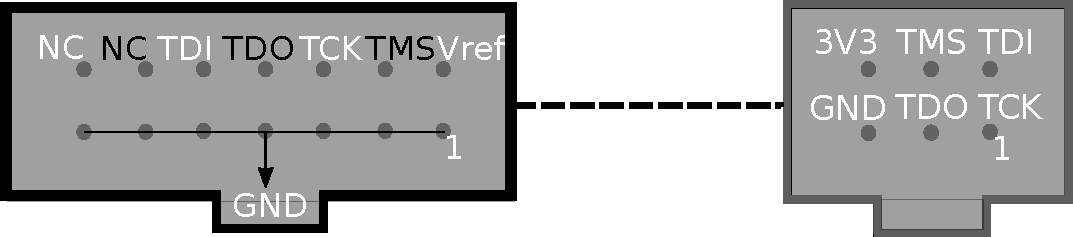
\includegraphics[width=0.9\linewidth]{Figures/data_cable}
	\caption{Programmierkabel HW-RIBBON14 zu 6 Pin IDC female}
	\label{fig:data_cable}
\end{figure}

In Abbildung \ref{fig:data_cable} erkennen Sie das favorisierte Datenkabel vom BitConnector zum Programmiergerät. Anders als in Abbildung \ref{fig:pinheader}, ist der 6 Pin Connector diesmal als Buchse ausgeführt und somit gespiegelt. Bei dem HW-RIBBON14 female connector hat sich Xilinx für eine eher exotische Buchse im 2 mm Raster entschieden. Die Kette des Datenkabels sieht abstrakt zusammen gefasst folgendermaßen aus:
\vspace{0.5cm}
\begin{center}
	PC<--USB-Kable-->Programmierer<--Programmierkabel-->BitConnector
\end{center}

\vspace{0.5cm}

Falls Sie kein passendes Kabel zur Hand haben, können Sie die herausgeführten JTAG Pins von den beiden Stiftleisten über ein Steckbrett abgreifen. Die passende Pinbelegung können Sie Kapitel \ref{sec:Pins} entnehmen.
Falls Sie mehrere BitConnectoren auf einer Platine gesockelt haben, bieten sich diese Pins ebenfalls an, um die CPLDs mit nur einer herausgeführten Schnittstelle sequenziell zu konfigurieren.


Für die Ansteuerung der JTAG-Schnittstelle wird ein Programmiergerät benötigt. Dieses gibt es in unterschiedlichen preislichen Ausführungen, wie das standard „Xilinx Platform Cable USB 1/II“, eine kleinere und günstigere Version für Universitäten „XUP USB-JTAG Programming Cable“ oder diverse sehr günstige Nachbauten zum DLC9G oder zum DLC9LP. 




%Die Pins „Global Clock“ und „Global Reset“ sind neben den klassischen I/O Pins Zusatzfunktionen, die erst softwareseitig in der „ISE“ aktiviert werden müssen.

\newpage
\printbibliography
\end{document}